\documentclass[11pt,a4paper]{article}
\usepackage[T1]{fontenc}
\usepackage[utf8]{inputenc}
\usepackage{lmodern}
\usepackage[margin=26mm]{geometry}
\usepackage{amsmath,amssymb,amsthm,mathtools}
\usepackage{booktabs,graphicx,microtype}
\usepackage{xcolor}
\usepackage[numbers,sort&compress]{natbib}
\usepackage[colorlinks=true,linkcolor=blue!45!black,citecolor=blue!45!black,urlcolor=blue!45!black]{hyperref}
\usepackage[font=small,labelfont=bf]{caption}
\hypersetup{pdftitle={A counterexample to the forward waiting-time entropy bound in periodically driven Markov networks},pdfauthor={Xiaojian Zeng}}
\newcommand{\dd}{\mathop{}\!\mathrm{d}}
\newcommand{\ts}{t_*}
\newcommand{\sigw}{\widehat{\sigma}_{\Psi}}
\newcommand{\sige}{\overline{\sigma}}
\newcommand{\V}{\mathcal{V}}
\newcommand{\T}{\mathcal{T}}
\newtheorem{proposition}{Proposition}
\DeclareMathOperator{\diag}{diag}
\setlength{\emergencystretch}{2em}
\title{A counterexample to the forward waiting-time entropy bound in periodically driven Markov networks}
\author{Xiaojian Zeng\\[3pt]
\small PBC School of Finance, Tsinghua University, Beijing 100190, China\\
\small\href{mailto:xiaojianzeng@foxmail.com}{xiaojianzeng@foxmail.com}}
\date{}
\begin{document}
\maketitle
\begin{abstract}
Waiting times between observable transitions can reveal dissipation in partially accessible Markov networks. For periodically driven networks, a proposed estimator compares phase-averaged waiting densities with the reversed event labels while retaining the same forward protocol. We give an exact counterexample to its conjectured universal upper bound by the physical entropy-production rate. The model has three states, one observable edge in both directions, and three successive constant-rate segments. Each segment satisfies detailed balance with the same uniform distribution, so all instantaneous probability currents and the specified system--bath entropy production vanish. Nevertheless, chronological ordering of the symmetric rates makes the two same-direction waiting densities different after the correct event-weighted phase average. For every fixed positive rate ratio other than one, we calculate a nonzero cubic short-delay coefficient and prove that the estimator is finite and strictly positive. For a rate ratio of ten, an explicit rational remainder bound certifies the sign, while an exponential survival estimate controls the entire waiting-time tail. Numerical propagation illustrates the signal but is not needed for the proof. The counterexample concerns time-dependent symmetric kinetic factors and does not include the implementation-dependent dissipation of an external protocol controller.
\end{abstract}
\noindent\textbf{Keywords:} stochastic thermodynamics; entropy inference; waiting-time distributions; periodic Markov processes; kinetic time ordering

\section{The forward-protocol inference question}
Observing a small set of transitions and their intervening waiting times can provide more information about dissipation than stationary currents alone. For time-independent Markov networks, transition-based waiting densities yield entropy-production bounds and recover the full dissipation of a single cycle observed through one edge pair \cite{vanderMeer2022}. Extending such inference to periodic driving requires specifying how both event labels and the driving protocol transform under time reversal.

Maier \emph{et al.}\ introduced a phase-averaged estimator using only the forward protocol and conjectured that it remains below the physical entropy-production rate \cite{Maier2024}. The relevant formulas are Eqs.~(17)--(18) of the published article; its Eq.~(16) is a different, proven bound involving the reversed protocol. Harunari \emph{et al.}\ likewise distinguish forward-only inference from bounds using reversed driving and additional phase information \cite{Harunari2024}. Here we disprove the universal upper bound for the forward-only estimator when positive, bounded, piecewise-continuous periodic rates are allowed.

The broader warning that waiting-time asymmetry can be mistaken for dissipation already has clear precedents. Blom \emph{et al.}\ exhibit a spurious waiting-time contribution under detailed balance for milestoned observations \cite{Blom2024}. A recent preprint by Schwarz, Hartich and Godec analyzes kinetic hysteresis in milestoning of Markov-jump dynamics (\href{https://arxiv.org/abs/2606.17033v1}{arXiv:2606.17033v1}, Secs.~I.2 and II). Our observation rule records the next event on a fixed microscopic edge pair; it does not retain a last-visited milestone as a coarse state. The specific contribution is an explicit periodic-rate counterexample to the estimator of Ref.~\cite{Maier2024}, together with its short-delay mechanism and complete normalization and integrability checks.

\section{Model, conventions and estimator}
Consider a finite connected bidirectional graph with positive, bounded, piecewise-continuous rates $k_{ij}(t)$ for $i\to j$, periodic with period $\T$, and a unique periodic distribution $p(t)$. We use column probabilities,
\begin{equation}
 \dot p=L(t)p,\qquad L_{ji}=k_{ij}\quad(i\ne j),\qquad
 L_{ii}=-\sum_{j\ne i}k_{ij}.
 \label{eq:master}
\end{equation}
Entropy is measured in units of Boltzmann's constant, and all logarithms are natural. The physical rate to be inferred is
\begin{equation}
 \sige=\frac1\T\int_0^\T\sum_{i\ne j}p_i(t)k_{ij}(t)
 \log\frac{p_i(t)k_{ij}(t)}{p_j(t)k_{ji}(t)}\dd t.
 \label{eq:entropy}
\end{equation}
The sum is over ordered edges, without an additional factor of $1/2$.
Local detailed balance fixes the ratio
$\log(k_{ij}/k_{ji})=F_i-F_j+f_{ij}$, with $f_{ij}=-f_{ji}$ and energies in bath-temperature units. This ratio condition alone does not require time-independent symmetric kinetic factors.

Let $\V$ be a visible directed-edge set closed under reversal, and let $\widetilde I$ denote the reversed label of $I$. Define
\begin{equation}
 n_I(t)=p_i(t)k_{ij}(t),\qquad
 \overline n_I=\frac1\T\int_0^\T n_I(t)\dd t,
 \qquad I=(i\to j).
 \label{eq:flux}
\end{equation}
The joint density of the next visible label $J$ and delay $\tau$, conditional on $I$ at phase $t$, is $\psi_{I\to J}(\tau\mid t)$. Thus its normalization is
\begin{equation}
 \sum_{J\in\V}\int_0^\infty\psi_{I\to J}(\tau\mid t)\dd\tau=1,
 \label{eq:jointnorm}
\end{equation}
and not a separate normalization for each $J$. Event-conditioned phase averaging gives \cite{Maier2024}
\begin{equation}
 \Psi_{I\to J}(\tau)=\frac{1}{\T\overline n_I}
 \int_0^\T n_I(t)\psi_{I\to J}(\tau\mid t)\dd t.
 \label{eq:average}
\end{equation}
The estimator under consideration is
\begin{equation}
 \sigw=\sum_{I,J\in\V}\overline n_I\int_0^\infty
 \Psi_{I\to J}(\tau)
 \log\frac{\Psi_{I\to J}(\tau)}{\Psi_{\widetilde J\to\widetilde I}(\tau)}\dd\tau.
 \label{eq:estimator}
\end{equation}
Both densities in the ratio refer to the same forward protocol. The question is whether $0\le\sigw\le\sige$ holds universally. A counterexample to its upper half suffices to answer this question negatively.

For completeness, these waiting laws can be calculated without a renewal assumption. Remove only the visible off-diagonal entries from $L$, retaining all escape diagonals:
\begin{equation}
 L_{\rm kill}(t)=L(t)-\sum_{(i\to j)\in\V}k_{ij}(t)|j\rangle\langle i|.
 \label{eq:killedgeneral}
\end{equation}
If $U_{\rm kill}(t',t)$ solves the corresponding column evolution, then
\begin{equation}
 \psi_{(i\to j)\to(k\to l)}(\tau\mid t)
 =k_{kl}(t+\tau)[U_{\rm kill}(t+\tau,t)]_{kj}.
 \label{eq:waiting}
\end{equation}
Equivalently, redirect each visible jump to its own absorbing state and read its absorption flux. This construction is used for periodic systems in Ref.~\cite{Harunari2024}, Sec.~V. Phase averaging does not by itself make successive intervals independent.

\section{A three-state protocol with zero physical dissipation}
Fix a time scale $\ts>0$, set $s=t/\ts$ and $x=\tau/\ts$, and take $r>0$. On the triangle define
\begin{equation}
 k_{12}=k_{21}=a(s)/\ts,\quad
 k_{23}=k_{32}=b(s)/\ts,\quad
 k_{31}=k_{13}=c(s)/\ts,
 \label{eq:rates}
\end{equation}
where the dimensionless rates repeat every three units:
\begin{equation}
 (a,b,c)(s)=
 \begin{cases}
 (r,1,1),&0\le s<1,\\
 (1,r,1),&1\le s<2,\\
 (1,1,r),&2\le s<3.
 \end{cases}
 \label{eq:protocol}
\end{equation}
Observe exactly $+=(1\to2)$ and $-=(2\to1)$; the other four directed jumps are hidden. All six rates lie between $\min(1,r)/\ts$ and $\max(1,r)/\ts$. They are piecewise constant, with period $\T=3\ts$. Values at isolated switching times do not affect the waiting integrals.

Every full generator is symmetric and conservative. Consequently
\begin{equation}
 p(t)=\tfrac13(1,1,1)^{\mathsf T},\qquad
 p_i k_{ij}=p_j k_{ji},\qquad \sige=0.
 \label{eq:zero}
\end{equation}
Each full segment propagator is strictly positive, so the stochastic product over a period has a unique normalized fixed point. The displayed distribution is therefore the unique periodic state. Local detailed balance holds with $F_i=f_{ij}=0$. In particular, there is no change of well energy at a switch and no discontinuity of $p$.

The two visible fluxes are equal, but their event phases are not uniformly distributed:
\begin{equation}
 n_+(t)=n_-(t)=\frac{a(s)}{3\ts},\qquad
 \overline n_+=\overline n_-=\frac{r+2}{9\ts},\qquad
 q(s)=\frac{a(s)}{r+2},\quad \int_0^3q(s)\dd s=1.
 \label{eq:phaseweight}
\end{equation}

\begin{proposition}
For the protocol \eqref{eq:protocol} and the specified visible edge pair, the estimator \eqref{eq:estimator} is finite and strictly positive for every fixed $r>0$ with $r\ne1$, whereas \eqref{eq:entropy} is exactly zero. At $r=1$, the estimator is zero. In particular, the proposed universal upper bound $\sigw\le\sige$ fails.
\label{prop:main}
\end{proposition}

The proof below is exact for this finite-state model. It uses neither an adiabatic limit nor a perturbative truncation of the estimator. A short-delay expansion is used only to identify an interval on which its nonnegative integrand is strictly positive.

\section{Why the forward waiting densities differ}
The dimensionless killed matrices are
\begin{equation}
 S(a,b,c)=
 \begin{pmatrix}
 -a-c&0&c\\
 0&-a-b&b\\
 c&b&-b-c
 \end{pmatrix}.
 \label{eq:S}
\end{equation}
Write $S_0,S_1,S_2$ for the three segments, and let $U(s+x,s)$ be their chronologically ordered column propagator. Introduce dimensionless same-direction densities
\begin{equation}
 A(x)=\ts\Psi_{+\to+}(\ts x),\qquad
 B(x)=\ts\Psi_{-\to-}(\ts x).
 \label{eq:AB}
\end{equation}
The initial states after the first event are respectively 2 and 1; the departure states of the next same-direction event are 1 and 2. Equations~\eqref{eq:average} and \eqref{eq:phaseweight} therefore give
\begin{equation}
 A(x)-B(x)=\frac1{r+2}\int_0^3 a(s)a(s+x)
 \bigl[U_{12}(s+x,s)-U_{21}(s+x,s)\bigr]\dd s.
 \label{eq:ABint}
\end{equation}
Under $(I,J)\mapsto(\widetilde J,\widetilde I)$ the mixed channels $(+,-)$ and $(-,+)$ each map to themselves. Their logarithms vanish. Pairing the other two terms, with the equal fluxes in \eqref{eq:phaseweight}, yields
\begin{equation}
 \ts\sigw=\frac{r+2}{9}\int_0^\infty
 (A-B)\log\frac AB\dd x.
 \label{eq:paired}
\end{equation}
For positive $A,B$, the integrand is nonnegative at every delay.

For $0<x<1$, a waiting interval crosses at most one switch. A no-switch interval contributes zero to \eqref{eq:ABint}, since $\exp(xS_i)$ is symmetric. For a switch $i\to j=i+1\pmod3$, located $u$ units after the first event,
\begin{equation}
 U(s+x,s)=e^{(x-u)S_j}e^{uS_i},\qquad 0<u<x.
 \label{eq:switchU}
\end{equation}
The endpoint weight is the constant $a_i a_j$. With $M_{12-21}=M_{12}-M_{21}$,
\begin{equation}
 A-B=\frac1{r+2}\sum_{i=0}^2a_i a_j\int_0^x
 \bigl[e^{(x-u)S_j}e^{uS_i}\bigr]_{12-21}\dd u.
 \label{eq:crossing}
\end{equation}
The wraparound switch $2\to0$ is included. Absolute convergence of the finite-matrix exponential series permits termwise integration, giving
\begin{equation}
 \int_0^xe^{(x-u)S_j}e^{uS_i}\dd u
 =\sum_{d=0}^{\infty}\frac{x^{d+1}}{(d+1)!}
 \sum_{m=0}^{d}S_j^mS_i^{d-m}.
 \label{eq:series}
\end{equation}
The terms $d=0,1$ have no antisymmetric component. At $d=2$, that component is $[S_j,S_i]_{12}x^3/6$. Direct multiplication gives
\begin{equation}
 \begin{split}
 a_0a_1[S_1,S_0]_{12}&=-r(r-1),\\
 a_1a_2[S_2,S_1]_{12}&=(r-1)(r+1),\\
 a_2a_0[S_0,S_2]_{12}&=-r(r-1).
 \end{split}
 \label{eq:commutators}
\end{equation}
Their sum is $-(r-1)^2$, and hence
\begin{equation}
 \boxed{\displaystyle
 A(x)-B(x)=-\frac{(r-1)^2}{6(r+2)}x^3+O(x^4),\qquad x\downarrow0.}
 \label{eq:cubic}
\end{equation}
For each fixed $r\ne1$, this coefficient is nonzero. The remainder constant may depend on $r$. Once positive support and convergence of \eqref{eq:paired} are established, \eqref{eq:cubic} proves strict positivity. For $r=1$, all three killed matrices coincide and $U$ is symmetric at every delay, so $A=B$ exactly. The nonzero signal for $r\ne1$ comes from the ordering of symmetric matrices, not from an instantaneous probability current.

\section{Joint normalization and the infinite-delay integral}
Let $m=\min(1,r)>0$ and $M=\max(1,r)$, and define
\begin{equation}
 K=\begin{pmatrix}2&0&-1\\0&2&-1\\-1&-1&2\end{pmatrix}.
 \label{eq:K}
\end{equation}
For every segment,
\begin{equation}
 \begin{split}
 -S-mK={}&(a-m)\diag(1,1,0)\\
 &+(b-m)(e_2-e_3)(e_2-e_3)^{\mathsf T}\\
 &+(c-m)(e_1-e_3)(e_1-e_3)^{\mathsf T}\succeq0.
 \end{split}
 \label{eq:quadratic}
\end{equation}
The leading principal minors of $K-\tfrac12 I$ are $3/2$, $9/4$ and $3/8$. Thus $-S\succeq(m/2)I$ as a quadratic-form bound. Applying the energy estimate to each segment and using continuity at switches gives
\begin{equation}
 \|U(s+x,s)\|_2\le e^{-mx/2}.
 \label{eq:contraction}
\end{equation}
For an initial unit mass, the remaining survival probability is at most $\sqrt3e^{-mx/2}$. Its loss rate equals the sum of the two visible absorption fluxes because the escape diagonals in \eqref{eq:S} were retained. Survival tends to zero, proving \eqref{eq:jointnorm} at every initial phase. Averaging with $q$ preserves this joint normalization.

The same bound gives $A,B\le M e^{-mx/2}$. To bound them from below, retain precisely two hidden jumps, $2\to3\to1$ for $A$ or $1\to3\to2$ for $B$, followed by the specified visible jump at $x$. Each of the three rate factors is at least $m$. The total escape rate is at most $2M$, and the ordered pair of hidden jump times has integration volume $x^2/2$. Uniformly in the initial phase,
\begin{equation}
 \frac{m^3x^2}{2}e^{-2Mx}\le A(x),B(x)\le M e^{-mx/2},\qquad x>0.
 \label{eq:genericbounds}
\end{equation}
In particular, both laws have positive support for every positive delay. Their ratio satisfies
\begin{equation}
 \left|\log\frac AB\right|\le
 \log\frac{2M}{m^3}+\left(2M-\frac m2\right)x-2\log x.
 \label{eq:logbounds}
\end{equation}
Together with the exponential upper bound, this controls the absolute integrand of \eqref{eq:paired}. The logarithmic singularity is integrable at zero and the tail decays exponentially. The estimator is therefore finite for every fixed $r>0$. Equation~\eqref{eq:cubic} now completes the proof of Proposition~\ref{prop:main}. None of these estimates is asserted to be uniform as $r$ tends to zero or infinity.

\section{An explicit sign bound and numerical illustration}
\subsection{A rational certificate at \texorpdfstring{$r=10$}{r=10}}
For $r=10$, the three killed matrices are
\begin{equation}
 \begin{split}
 S_0&=\begin{pmatrix}-11&0&1\\0&-11&1\\1&1&-2\end{pmatrix},\qquad
 S_1=\begin{pmatrix}-2&0&1\\0&-11&10\\1&10&-11\end{pmatrix},\\[3pt]
 S_2&=\begin{pmatrix}-11&0&10\\0&-2&1\\10&1&-11\end{pmatrix}.
 \end{split}
 \label{eq:matrices10}
\end{equation}
Their induced infinity norms are $12,22,22$, and their endpoint weights in \eqref{eq:crossing} sum to $21$. The weighted commutator entries are $-90,99,-90$, giving $A-B=-9x^3/8+R(x)$. Bounding an antisymmetric entry by twice an induced matrix norm in \eqref{eq:series},
\begin{equation}
 |R(x)|\le\frac72x\sum_{d\ge3}\frac{(22x)^d}{d!}
 \le\frac7{12}22^3x^4e^{22x}.
 \label{eq:remainder}
\end{equation}
Set $\delta=1/20000$. Since $e^y\le(1-y)^{-1}$ for $0\le y<1$,
\begin{equation}
 \frac{|R(x)|}{x^3}\le
 \frac{(7/12)22^3\delta}{1-22\delta}
 =\frac{1331}{4281}<\frac9{16},\qquad 0<x\le\delta.
 \label{eq:remainderconstant}
\end{equation}
Consequently $B-A\ge9x^3/16$ on this interval. Also $A,B\le10$, and the mean-value formula for the logarithm gives
\begin{equation}
 (A-B)\log(A/B)\ge\frac{(A-B)^2}{\max(A,B)}.
 \label{eq:logmv}
\end{equation}
Using the nonnegativity of the integrand outside $(0,\delta]$, we obtain
\begin{equation}
 \ts\sigw\ge\frac43\frac1{10}\left(\frac9{16}\right)^2\frac{\delta^7}{7}
 =\frac{27}{4480\cdot20000^7}>0.
 \label{eq:rational}
\end{equation}
This deliberately small bound, approximately $4.71\times10^{-33}$, certifies a strict sign; it does not estimate the actual signal magnitude.

Here the escape rate is at most $11$, improving \eqref{eq:genericbounds} to
\begin{equation}
 \frac{x^2}{2}e^{-11x}\le A,B\le10e^{-x/2}.
 \label{eq:bounds10}
\end{equation}
For $H\ge1$, the remaining dimensionless entropy integral obeys
\begin{equation}
 \frac43\int_H^\infty(A-B)\log(A/B)\dd x
 \le\frac{80}{3}e^{-H/2}\bigl(2\log20+22H+44\bigr).
 \label{eq:tail}
\end{equation}
Indeed, $|A-B|\le A+B\le20e^{-x/2}$ and
$|\log(A/B)|\le\log20+(21/2)x-2\log x\le\log20+11x$ on this domain. At $H=80$, \eqref{eq:tail} is below $2.051\times10^{-13}$, and each missing joint probability is at most $\sqrt3e^{-40}<7.359\times10^{-18}$. The tail bound is not subtracted from \eqref{eq:rational}: that exact sign argument already uses the nonnegative integrand on the full domain.

\subsection{Propagation checks and signal size}
Three finite-matrix calculations check the waiting laws: chronological three-state matrix exponentials; a separately constructed five-state absorbing chain integrated with DOP853; and a five-state Poisson uniformization calculation. Figure~\ref{fig:waiting} illustrates the two same-direction densities. Phase quadrature is split wherever the initial or final phase crosses a switch, and delay quadrature is split at integer $x$. No channel is rescaled to unit mass.

\begin{figure}[tb]
 \centering
 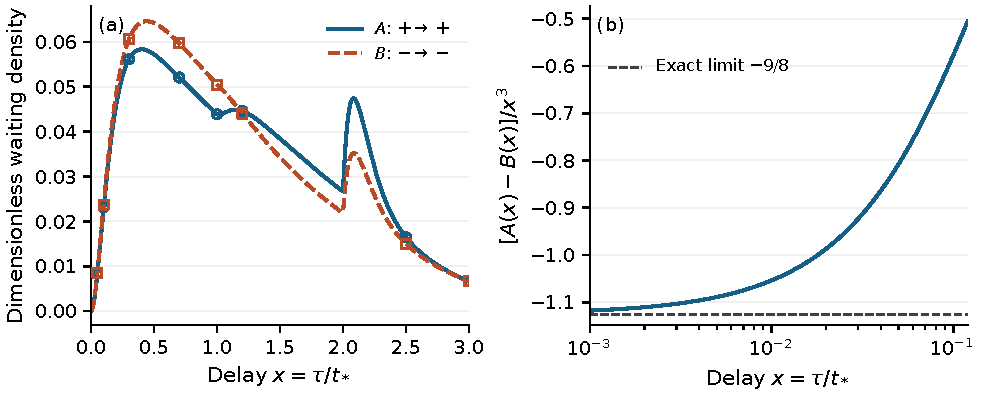
\includegraphics[width=\textwidth]{figures/waiting.pdf}
 \caption{Same-direction waiting laws for $r=10$. (a) Dimensionless densities $A$ and $B$ from the killed propagator with 32-point Gauss phase quadrature. Markers show the separately constructed absorbing-chain ODE calculation at the indicated delays. (b) The short-delay difference divided by $x^3$; the horizontal line is the exact limit $-9/8$ from \eqref{eq:cubic}. Curves are floating-point illustrations, not interval certificates. The physical entropy-production rate is exactly zero throughout this protocol.}
 \label{fig:waiting}
\end{figure}

At $r=10$, the numerical estimate is $\sigw\simeq0.0030163/\ts$. Table~\ref{tab:numeric} records diagnostic convergence at $H=80$. The maximum dimensionless density discrepancy between the ODE and exponential implementations is below $1.16\times10^{-12}$ over 12 sampled delays from $0.001$ to $10$. The Poisson calculation uses degree 85 with rate 11 on subsegments of length at most one; its per-subsegment omitted Poisson mass is below $2.865\times10^{-46}$. This controls that series truncation only, not the floating-point or Gauss-quadrature errors. The displayed decimals are thus numerical diagnostics, while strict positivity and the infinite-domain existence follow from the preceding analysis.

\begin{table}[tb]
\centering
\caption{Dimensionless estimator at $r=10$, with delay cutoff $H=80$. The same Gauss order $q$ is used for phase and delay on their respective smooth subintervals. The normalization error is the maximum absolute deviation of an integrated joint row sum from one. All displayed decimals are rounded approximations to floating-point diagnostics.}
\label{tab:numeric}
\begin{tabular}{lrrr}
\toprule
Propagation & $q$ & $\ts\sigw$ (diagnostic) & Normalization error\\
\midrule
Matrix exponentials & 20 & 0.003016257369842 & $1.00\times10^{-14}$\\
Matrix exponentials & 32 & 0.003016257524653 & $1.04\times10^{-14}$\\
Matrix exponentials & 64 & 0.003016257524685 & $7.55\times10^{-15}$\\
Poisson uniformization & 16 & 0.003016254883273 & $2.00\times10^{-15}$\\
Poisson uniformization & 24 & 0.003016257515582 & $<9\times10^{-15}$\\
\bottomrule
\end{tabular}
\end{table}

Additional checks recover $A=B$ for $r=1$, exchange the same-direction densities under protocol reversal, and preserve the phase-averaged laws under a cyclic shift of the phase origin. A time-independent single-cycle benchmark is given in Appendix~\ref{app:baseline}. Reproduction scripts, the numerical data and regeneration instructions accompany the manuscript; the largest matrix is $5\times5$, and no stochastic sampling is used.

\section{Physical interpretation and scope}
Instantaneous detailed balance makes each killed matrix symmetric, but a chronological product of different symmetric matrices need not be symmetric. In this protocol the first surviving phase-averaged antisymmetric contribution is the sum of three switch commutators. Event-conditioned sampling weights these switches by the endpoint rates, producing the nonzero coefficient \eqref{eq:cubic}. Thus forward waiting statistics retain information about kinetic temporal ordering even though the probabilities remain uniform and the prescribed physical dissipation is zero.

The example varies symmetric kinetic factors while leaving all rate ratios equal to one. The general periodic-rate formulation and local-detailed-balance condition in Ref.~\cite{Maier2024}, Sec.~2, permit such variation; the fixed kinetic prefactors in its Appendix~A specify a narrower numerical test family. Our counterexample concerns the general estimator and rate domain. It does not establish a counterexample within a fixed-prefactor parametrization or for smooth driving. No smoothing argument is required because the stated domain includes piecewise-continuous protocols.

This failure also does not challenge the time-independent results of Ref.~\cite{vanderMeer2022} or the reversed-protocol bound of Ref.~\cite{Maier2024}. Reversing event labels within a forward experiment is a different operation from reversing the order of the externally imposed rates. Nor does the argument establish or refute a universal lower inequality $0\le\sigw$ in arbitrary periodic networks: nonnegativity here follows from the equal-flux pairing \eqref{eq:paired} for this particular observation set.

Finally, \eqref{eq:entropy} is the stated finite-state system--bath entropy-production rate. The physical realization of the external barrier controller is not part of this model and can have additional dissipation. The conclusion is consequently about the thermodynamic meaning of this forward-data estimator under its specified target observable, not about a costless autonomous clock or an experimental observation. Even with full waiting-time resolution on the visible edge pair, a positive value of \eqref{eq:estimator} alone cannot provide the proposed universal lower estimate of \eqref{eq:entropy}.

\appendix
\section{Time-independent single-cycle benchmark}
\label{app:baseline}
As a check on direction conventions and joint normalization, take a stationary three-state ring with clockwise rates $2/\ts$ and counterclockwise rates $1/\ts$, observing the same edge pair. The periodic notation then reduces to a time-independent uniform state. The full entropy-production rate is $\log2/\ts$. The dimensionless killed matrix is
\begin{equation}
 S_{\rm st}=\begin{pmatrix}-3&0&2\\0&-3&1\\1&2&-3\end{pmatrix}.
\end{equation}
For dimensionless waiting densities, $A(x)=2[e^{xS_{\rm st}}]_{12}$ and $B(x)=[e^{xS_{\rm st}}]_{21}$. The diagonal matrix $D=\diag(1,1/2,1/\sqrt2)$ makes $D^{-1}S_{\rm st}D$ symmetric. It follows that $[e^{xS_{\rm st}}]_{12}/[e^{xS_{\rm st}}]_{21}=4$ and hence $A/B=8$ for $x>0$. Integrating the four channels using $\int_0^\infty e^{xS_{\rm st}}\dd x=-S_{\rm st}^{-1}$ yields
\begin{equation}
 \left(\int_0^\infty\Psi_{I\to J}(\tau)\dd\tau\right)_{I,J=+,-}
 =\begin{pmatrix}8/15&7/15\\14/15&1/15\end{pmatrix}.
 \label{eq:benchmark}
\end{equation}
With $\overline n_+=2/(3\ts)$ and $\overline n_-=1/(3\ts)$, the estimator is
\begin{equation}
 \sigw=\frac1\ts\left(\frac23\frac8{15}-\frac13\frac1{15}\right)\log8
 =\frac{\log2}{\ts}.
\end{equation}
This reproduces the known single-cycle equality in Ref.~\cite{vanderMeer2022}, Sec.~III, and is a benchmark rather than a new result.

\section*{Statements and declarations}
\paragraph{Data and code availability.}
The accompanying reproducibility material contains the exact algebra checks, the finite-state propagation implementations, the numerical data underlying the figure and table, and build and regeneration instructions. The central result is the self-contained analytic argument above and does not depend on an external dataset.

\paragraph{Use of generative artificial intelligence.}
OpenAI Codex was used in developing the candidate protocol and arguments, carrying out symbolic and numerical calculations, producing and checking code, screening literature, and drafting the manuscript. Its use extended beyond copy editing. An additional AI verification pass reconstructed the source inputs and checked the result with a separate propagation implementation. These checks do not constitute external peer review. Human scientific review and final author approval of this draft remain pending.

\bibliographystyle{unsrtnat}
\bibliography{references}
\end{document}
